\documentclass{beamer}
\usepackage{graphicx} \usepackage[export]{adjustbox} \usepackage{float}
\usepackage{amsmath,amssymb,amsfonts}
\newcommand{\eqline}[1]{~\vspace{0.1cm}\\\centerline{$#1$}\vspace{0.1cm}\\}
\newcommand{\defq}{\stackrel {\rm def}{=}}
\newcommand{\tab}{\hphantom{4mm}}

\title{Programmatoid and neuronoid computations}
\author{Nicolas Rougier et al}
\begin{document}
\iffalse
\frame{\titlepage}

\begin{frame}
\frametitle{What about ?}
\centerline{\Huge {\em Programming} (not training)}
\centerline{\Huge neural networks}
{\huge  ~\\ \begin{itemize}
  \item With a benchmark and …
  \item Using computer algebra.
\end{itemize}} \end{frame}

\begin{frame}
  \frametitle{But … why ?}  {\Large  ~\\ \begin{itemize}
  \item For the fun :)
  \item To illustrate  a feed-forward neural network computational property.
  \item To provide an approximate neural network complexity  lower bound, given a task.
  \item To obtain a parsimonious computation tool.
  \item Why not ?
\end{itemize}} \end{frame}

\begin{frame}
\frametitle{The braincraft benchmark}
\centerline{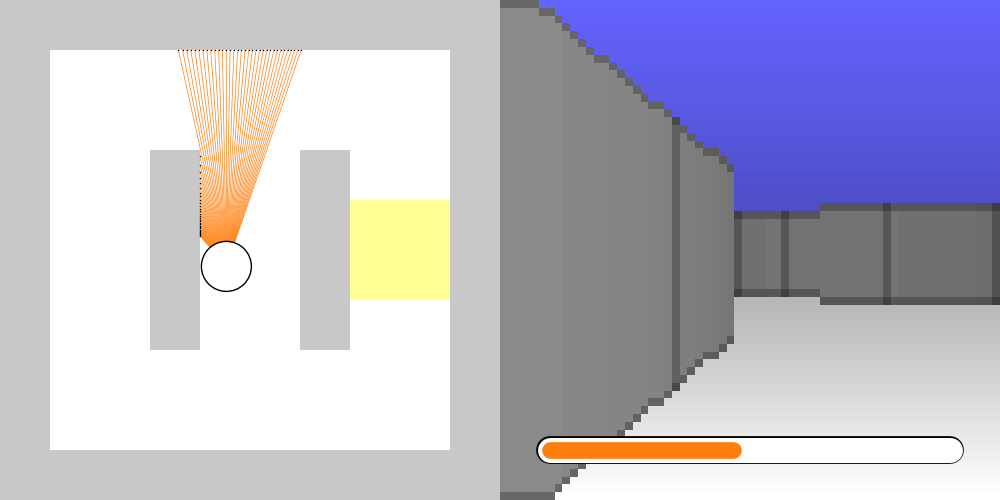
\includegraphics[width=0.9\textwidth]{../../data/debug.png}}
\end{frame}

\begin{frame}
  \frametitle{Three tasks:}
  \begin{tabular}{|l|l|l|}\hline
    \parbox[t]{0.25\textwidth}{\href{http://nowhere}{Find the energy source leftward or rightward}.} &
    \parbox[t]{0.25\textwidth}{\href{http://nowhere}{Find the correct direction, given the blue cue}.} &
    \parbox[t]{0.25\textwidth}{\href{http://nowhere}{FChoose the best energy source}.} \\
\hline\end{tabular} \end{frame}

\begin{frame}
  \frametitle{A (simplified) bot, with:}
  \centerline{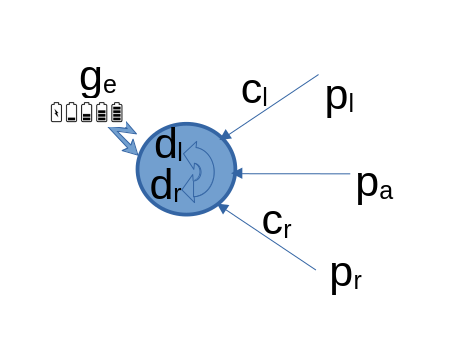
\includegraphics[width=0.5\textwidth]{./bot.png}}
  ~\\- left, ahead and right proximity sensors \\ \tab  \tab  \tab  \tab $p_\bullet \in  ]0_{\mbox{no-wall}}, 1_{\mbox{wall-hit}}], \bullet \in \{l, a, r\}$, \\- color sensors $c_{\bullet\dagger}$, \\- energy gauge $g_e \in [0_{\mbox{death}}, 1_{\mbox{full}}]$, \\- running at constant velocity, and \\-turning leftward or rightward $d_l \in [0, 1_{+ 5^o}]$.
\end{frame}

\fi

\begin{frame}
  \frametitle{Heuristics:}
  \centerline{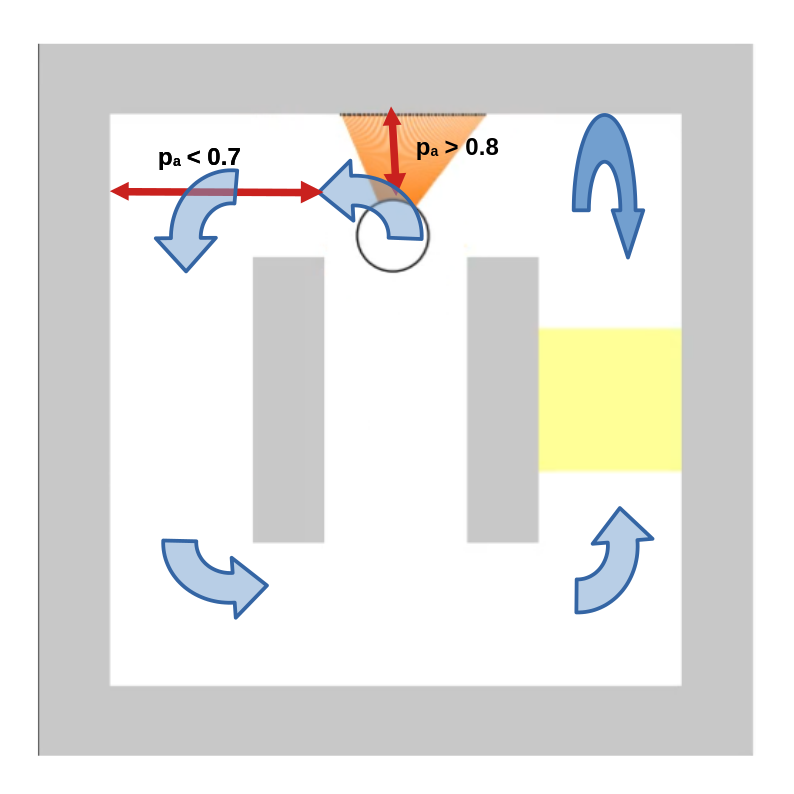
\includegraphics[width=0.4\textwidth]{./navigation.png} \tab 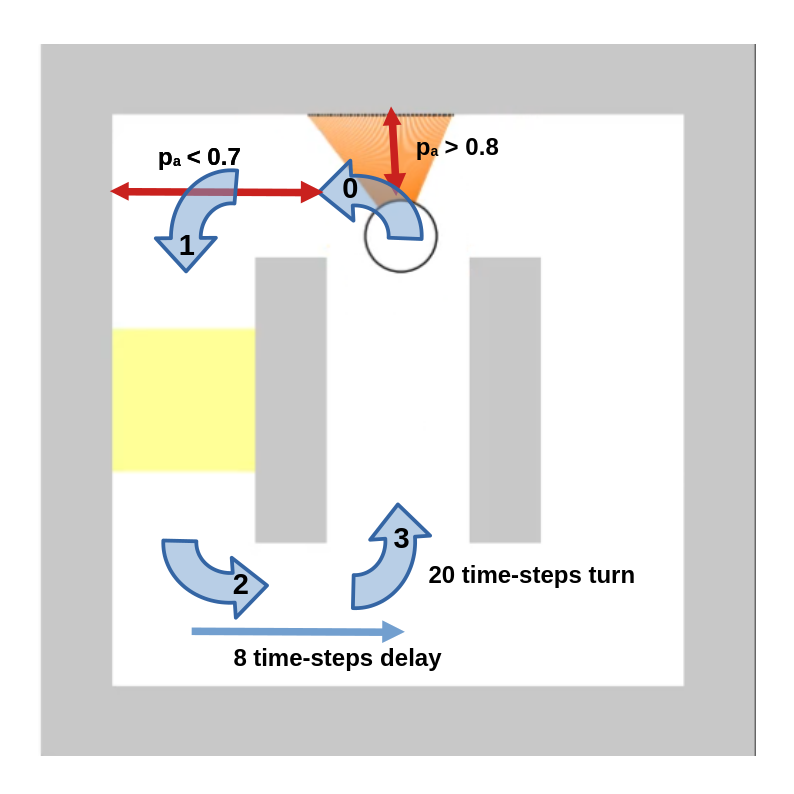
\includegraphics[width=0.4\textwidth]{./navigation2.png}}  \begin{itemize}
    \item Stabilizes the forward motion using linear feedback correction.
    \item Performs quarter-turn using ahead proximity thresholds.
    \item Performs about-turn or half-corridor turn using delays.
    \item Stores the preferred quarter-turn direction, e.g. from cue.
    \item Stores previous energy feeds for comparison.
\end{itemize}\end{frame}
\end{document}


\begin{frame}
  \frametitle{Programmatic implementation:}
\end{frame}
\end{document}
